\documentclass{article}

\usepackage{hyperref}
\usepackage{textcomp}
\usepackage{xcolor}
\usepackage{soul}
\usepackage{graphicx}

\definecolor{cmd}{RGB}{210,210,210}
\newcommand{\consolecommand}[1]{
\begingroup%
  \sethlcolor{cmd}%
  \hl{\texttt{#1}}%
\endgroup}
%\newcommand{\clickthis}[1]{\textbf{''#1''}}
%\newcommand{\pathfmt}[1]{\textbf{#1}}

\title{Jupyter Notebooks: Installation and Usage}
\author{Semantic Web}

\begin{document}
	\maketitle
	\section{Introduction}
	In our lecture \emph{Semantic Web}, we will use \emph{Jupyter Notebooks} as assignments. There are many different ways to edit and run jupyter notebooks and in this document we will show you two of them. The first way is to install a local notebook server. The second way is to use the \emph{RWTH JupyterHub}. In the following sections we will guide you through both processes step-by-step. In case one of these methods does not work for you, you can still try the other one.
	

	\section{Local Installation using Anaconda}
	If you choose to use a local notebook server, it is highly recommended to use a brand new virtual environment with the latest python version.
	Install \href{https://www.anaconda.com/products/individual#Downloads}{Anaconda} if you haven't already. Then create a new virtual environment with \consolecommand{conda create --name semweb}. Every time you want to use the virtual environment you have to activate it with \consolecommand{conda activate semweb}. Activate the environment if you haven't already. Then install jupyter notebook and the graphviz interface with \consolecommand{conda install -c conda-forge notebook python-graphviz ipython=7.18.1}. Change into your desired notebook directory and start the notebook server with \consolecommand{jupyter notebook}. After that command a webbrowser with the notebook interface should open. To open a notebook, just copy it into your directory and double click it in the webbrowser.
%	\subsection{Python}
%	For this lecture you will need \href{https://graphviz.org/download/}{GraphViz}. The anaconda package also contains the graphviz binaries but when using stock python you also need to install graphviz and add its binary directory to the path.
%	Because the activation of virtual environments with virtualenv is platform specific we will not cover it here, please consult \href{https://packaging.python.org/guides/installing-using-pip-and-virtual-environments/}{this guide}. After activating your virtual environment, install jupyter notebook and the graphviz interface with \consolecommand{python -m pip install notebook graphviz}. Change into your desired notebook directory and start the notebook server with \consolecommand{jupyter notebook}. After that command a webbrowser with the notebook interface should open. To open a notebook, just copy it into your directory and double click it in the webbrowser.
	\section{Using JupyterHub}
	\begin{figure}[t]
		\centering
		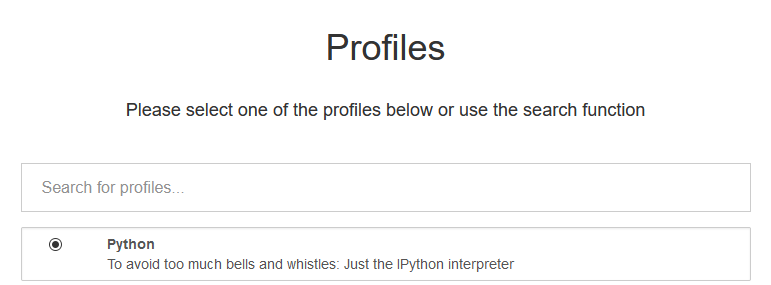
\includegraphics[width=.8\textwidth]{img/profiles.png}
		\caption{Profile selection screen. Just choose Python and click start at the bottom of the page.}
		\label{fig:profiles}
	\end{figure}
	Visit the \href{https://jupyter.rwth-aachen.de/hub/login}{\emph{RWTH JupyterHub}}, then login with your RWTH Shibboleth credentials. You will then be presented the profile selection screen shown in \ref{fig:profiles}. Just choose the Python profile -- should be the top one -- and click the start button at the bottom of the page to continue. Your Jupyter Notebook server will then be started up, which may take some seconds. After this you will be taken to the \emph{JupyterLab} interface of your server shown in \ref{fig:jupyterlab}.

	
	To open a notebook in JupyterLab, you first need to upload it. On the left side of the screen should be a file browser. If it isn't there, click the folder icon on the top left. There are already some folders but ignore these for now as they are not important. To upload a file, either drag and drop it from a file explorer into the file browser of the JupyterLab or click the upload file button at the top of the file browser (small arrow pointing up) and then choose the assignment's notebook file (ends in .ipynb). After you uploaded the notebook you just have to double click it in the file browser to open it.

	\begin{figure}[b]
	\centering
	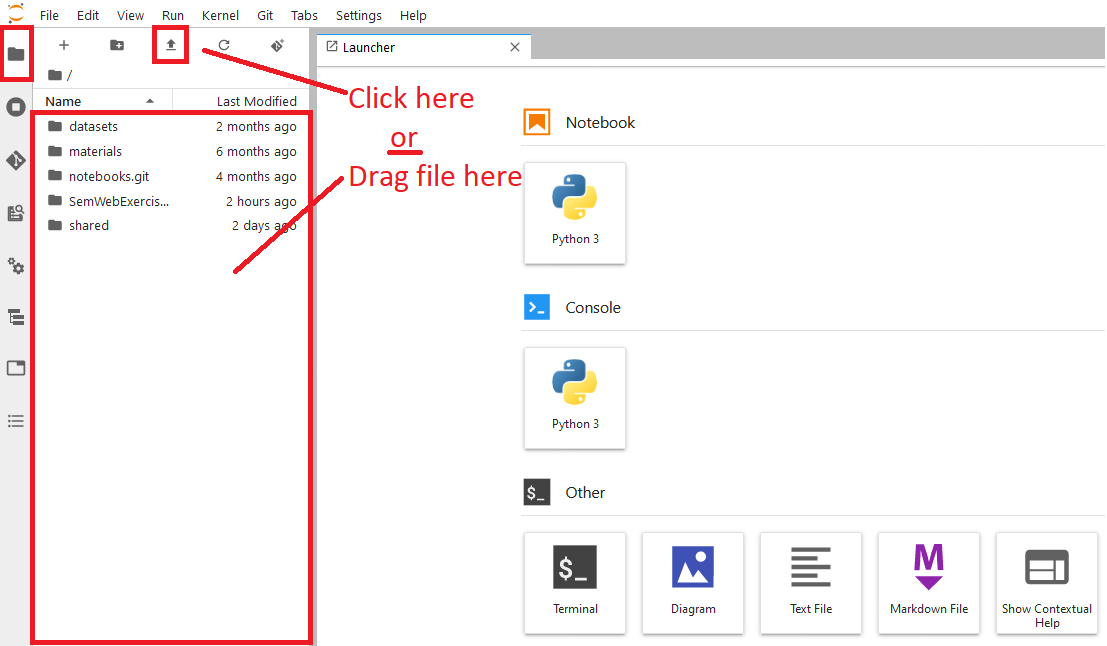
\includegraphics[width=\textwidth]{img/jupyterlab.png}
	\caption{JupyterLab interface. Upload a file by either dragging it into the file browser or clicking upload file. If the file browser isn't there, click the folder icon in the top left.}
	\label{fig:jupyterlab}
	\end{figure}
	
	
	
\end{document}